\documentclass[tikz,border=2mm]{standalone}
\usetikzlibrary{arrows.meta, positioning}

\begin{document}

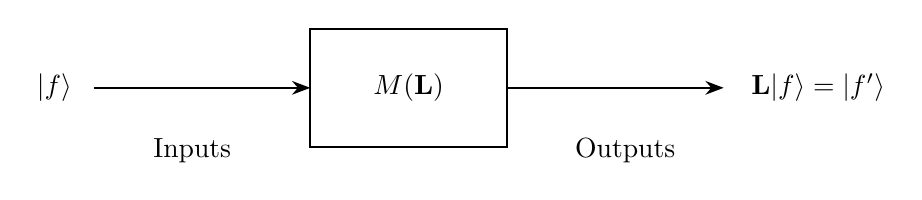
\begin{tikzpicture}[
    block/.style={
        rectangle,
        draw,
        minimum width=2.5cm,
        minimum height=1.5cm,
        thick
    },
    arrow/.style={
        ->,
        thick,
        >=Stealth
    }
]

% Central block
\node[block] (system) at (0,0) {$M(\mathbf{L})$};

% Input arrow and labels
\draw[arrow] (-4,0) -- (-1.25,0);
\node at (-4.5,0) {$|f\rangle$};
\node at (-2.75,-0.8) {Inputs};

% Output arrow and labels
\draw[arrow] (1.25,0) -- (4,0);
\node at (5.2,0) {$\mathbf{L}|f\rangle = |f'\rangle$};
\node at (2.75,-0.8) {Outputs};

\end{tikzpicture}

\end{document}